\documentclass[11pt,a4paper,oneside]{report}

% ======================================================================
% Agentic, Offline, and Private: A Local RAG-SQL System for
% University Data Management -- Major Project Report
% ======================================================================

\usepackage[margin=1in]{geometry}
\usepackage{fontspec}
\setmainfont{Latin Modern Roman}
\newfontfamily\monofont{Latin Modern Mono}
\usepackage{titlesec}
\usepackage{enumitem}
\usepackage{fancyhdr}
\usepackage{xcolor}
\usepackage{hyperref}
\usepackage{tabularx}
\usepackage{longtable}
\usepackage{tikz}
\usetikzlibrary{positioning,fit,arrows.meta}
\usepackage{listings}
\usepackage{xurl}
\usepackage{colortbl}
\usepackage{setspace}
\usepackage{caption}

\definecolor{hdrnavy}{RGB}{31,55,86}
\definecolor{hdrblue}{RGB}{224,232,242}
\definecolor{rulegray}{RGB}{120,120,120}

\urlstyle{tt}

\hypersetup{
    colorlinks=true,
    linkcolor=black,
    citecolor=black,
    urlcolor=blue,
    pdftitle={Agentic, Offline, and Private: A Local RAG-SQL System for University Data Management},
    pdfauthor={Vikas Bhowate, Om Gawande, Yash Garad, Harshal Ninawe, Aanchal Kalambe, Aditi Parshivanikar},
    pdfsubject={Major Project Report}
}

% ---- chapter / section styling ------------------------------------------
\titleformat{\chapter}[display]
  {\normalfont\bfseries\Large}{\chaptertitlename\ \thechapter}{10pt}{\Large}
\titlespacing*{\chapter}{0pt}{0pt}{24pt}
\titleformat{\section}{\large\bfseries}{\thesection}{0.6em}{}
\titleformat{\subsection}{\normalsize\bfseries}{\thesubsection}{0.6em}{}

\setlength{\headheight}{14pt}
\pagestyle{fancy}
\fancyhf{}
\fancyhead[L]{\small\itshape Agentic, Offline, and Private}
\fancyhead[R]{\small\thepage}
\renewcommand{\headrulewidth}{0.4pt}

\setlist[enumerate,1]{label=\arabic*.}

% ---- code-listing style -------------------------------------------------
\lstdefinestyle{codebox}{
    basicstyle=\monofont\scriptsize,
    numbers=left,
    numberstyle=\tiny\color{gray},
    numbersep=6pt,
    breaklines=true,
    breakatwhitespace=false,
    showstringspaces=false,
    tabsize=4,
    frame=single,
    rulecolor=\color{rulegray},
    framesep=4pt,
    columns=flexible,
    keepspaces=true,
    upquote=true,
    literate={—}{{---}}1 {…}{{\ldots}}1
}
\lstset{style=codebox}

\newcommand{\ReportTitle}{Agentic, Offline, and Private: A Local RAG--SQL System for University Data Management}

\begin{document}

% =====================================================================
% FRONT MATTER
% =====================================================================
\pagenumbering{roman}
\pagestyle{empty}

% ---- Title page -----------------------------------------------------
\begin{titlepage}
\begin{center}
\vspace*{1.2cm}
{\Large \bfseries \ReportTitle}\\[0.6cm]
{\normalsize \itshape A Project Report}\\[1.8cm]

{\normalsize Submitted in partial fulfilment of the requirements for the degree of}\\[0.2cm]
{\normalsize \bfseries Bachelor of Engineering}\\
{\normalsize in}\\
{\normalsize \bfseries Computer Science and Engineering}\\[1.6cm]

{\normalsize \bfseries By}\\[0.4cm]
{\normalsize
Mr.\ Om Gawande \\
Mr.\ Yash Garad \\
Mr.\ Harshal Ninawe \\
Ms.\ Aanchal Kalambe \\
Ms.\ Aditi Parshivanikar \\
}
\vspace{0.4cm}

{\normalsize \bfseries Under the guidance of}\\[0.3cm]
{\normalsize Dr.\ Vikas Bhowate}\\[1.6cm]

{\normalsize \bfseries Department of Computer Science and Engineering}\\[0.3cm]
\rule{6.5cm}{0.4pt}\\
{\small \itshape (Institute name)}\\[1.2cm]

{\normalsize Academic Year 2025--2026}
\end{center}
\end{titlepage}

% ---- Certificate ------------------------------------------------------
\thispagestyle{empty}
\begin{center}
{\Large \bfseries CERTIFICATE}
\end{center}
\vspace{1cm}

\noindent This is to certify that the project report entitled \textbf{``\ReportTitle''}
is a bona fide record of the work carried out by

\begin{center}
\begin{tabular}{ll}
Mr.\ Om Gawande & \rule{4cm}{0.4pt} \\[0.3cm]
Mr.\ Yash Garad & \rule{4cm}{0.4pt} \\[0.3cm]
Mr.\ Harshal Ninawe & \rule{4cm}{0.4pt} \\[0.3cm]
Ms.\ Aanchal Kalambe & \rule{4cm}{0.4pt} \\[0.3cm]
Ms.\ Aditi Parshivanikar & \rule{4cm}{0.4pt} \\[0.3cm]
\end{tabular}
\end{center}

\noindent under my supervision, in partial fulfilment of the requirements for
the degree of Bachelor of Engineering in Computer Science and Engineering, for
the academic year 2025--2026. The work presented in this report has not been
submitted elsewhere for the award of any other degree or diploma.

\vspace{2cm}
\begin{center}
\begin{tabular}{p{6cm}p{6cm}}
\rule{6cm}{0.4pt} & \rule{6cm}{0.4pt} \\
Dr.\ Vikas Bhowate & Head of Department \\
Project Guide & Computer Science and Engineering \\
\end{tabular}
\end{center}

\vspace{1.5cm}
\noindent Place: \rule{5cm}{0.4pt} \hfill Date: \rule{5cm}{0.4pt}

\clearpage

% ---- Declaration -------------------------------------------------------
\thispagestyle{empty}
\begin{center}
{\Large \bfseries DECLARATION}
\end{center}
\vspace{1cm}

\noindent We hereby declare that the project entitled \textbf{``\ReportTitle''}
is an original piece of work carried out by us under the guidance of Dr.\ Vikas
Bhowate, and that it has not been submitted, in whole or in part, for the
award of any other degree, diploma, or similar title at this or any other
institution. All sources of information used in this report have been duly
acknowledged.

\vspace{2cm}
\renewcommand{\arraystretch}{2.0}
\begin{tabularx}{\linewidth}{Xr}
Mr.\ Om Gawande & \rule{4cm}{0.4pt} \\
Mr.\ Yash Garad & \rule{4cm}{0.4pt} \\
Mr.\ Harshal Ninawe & \rule{4cm}{0.4pt} \\
Ms.\ Aanchal Kalambe & \rule{4cm}{0.4pt} \\
Ms.\ Aditi Parshivanikar & \rule{4cm}{0.4pt} \\
\end{tabularx}

\vspace{1cm}
\noindent Date: \rule{5cm}{0.4pt}

\clearpage

% ---- Acknowledgement ----------------------------------------------------
\thispagestyle{empty}
\begin{center}
{\Large \bfseries ACKNOWLEDGEMENT}
\end{center}
\vspace{1cm}

\noindent We express our sincere gratitude to our project guide, Dr.\ Vikas
Bhowate, for his continual guidance, technical insight, and encouragement
throughout the design, implementation, and evaluation of this project. His
emphasis on rigorous, verifiable engineering --- rather than superficial
demonstration --- shaped both the architecture of the system described in
this report and the discipline with which it was tested.

We also thank the Department of Computer Science and Engineering for
providing the infrastructure and environment necessary to carry out this
work, and our peers for their feedback during informal reviews of the system.

Finally, we acknowledge the open-source communities behind Django, React,
PostgreSQL, Qdrant, and Ollama, whose freely available tools made a fully
offline, self-hosted deployment of this scope achievable within an academic
project timeline.

\clearpage

% ---- Abstract ------------------------------------------------------------
\thispagestyle{empty}
\begin{center}
{\Large \bfseries ABSTRACT}
\end{center}
\vspace{0.8cm}

\noindent Institutions that want to let students and staff ask natural-language
questions about courses, faculty, fees, and schedules face an uncomfortable
choice: route those questions through a cloud large-language-model (LLM) API
and accept that institutional and student data leaves the campus network, or
forgo conversational access altogether. This project presents \emph{College
Assistant}, an agentic, fully offline question-answering system that resolves
this trade-off by running every stage of inference --- retrieval, SQL
generation, answer synthesis, and answer verification --- on
institution-controlled hardware, using open-weight models served locally by
Ollama.

The system decomposes what would otherwise be a single, over-trusted LLM call
into five cooperating agents: a router that classifies each question, a SQL
agent that generates and executes strictly read-only, schema-restricted
queries against the live institutional database, a retrieval-augmented
generation (RAG) agent that searches a locally hosted Qdrant vector store for
descriptive context, a synthesis agent that composes the final answer, and a
verification agent that checks the answer against its evidence before it is
returned. A dedicated web-fetch agent may consult a fixed, keyword-matched
allowlist of official institutional pages; the model is never permitted to
choose a URL. Generated SQL is independently parsed and validated by a guard
built on \texttt{sqlglot} before execution, and the database role available to
the model carries no write privileges and no access to personally
identifiable student records, so a fully compromised or adversarially
prompted model still cannot exfiltrate credentials, modify data, or read
another user's conversation.

The system was evaluated on commodity, GPU-less hardware (16 CPU cores, no
CUDA accelerator). Targeted optimisation of the routing and verification
stages reduced router latency by roughly four orders of magnitude (5.7\,s to
0.4\,ms) and cut short-answer verification latency from 11.3\,s to 50\,ms,
bringing end-to-end median response time for a seven-question benchmark down
from 1{,}455.8\,s to 876.7\,s while holding routing accuracy at 7/7 identical
routes. A follow-on scaling study identified model eviction between requests
as the single largest latency contributor (a 19.6$\times$ slowdown when the
LLM had to reload) and showed that a semantic answer cache alone does nothing
for simultaneous identical questions --- request coalescing was required to
take a 50-user, 5-question workload from 2 served requests per minute to all
50 succeeding at 28.1 requests/min.

The resulting system demonstrates that a multi-agent, defence-in-depth
architecture can deliver natural-language access to live institutional data
without a cloud dependency, without granting the language model direct write
or broad read access, and at a latency that, after optimisation, is usable on
hardware a mid-sized institution can reasonably own outright.

\vspace{0.8cm}
\noindent\textbf{Keywords:} Retrieval-Augmented Generation, Text-to-SQL,
Multi-Agent Systems, Local LLM Inference, Data Privacy, University Information
Systems, Ollama, Vector Search.

\clearpage

% ---- Table of contents ---------------------------------------------------
\pagestyle{fancy}
\setcounter{tocdepth}{1}
\makeatletter
\renewcommand*\l@chapter[2]{%
  \ifnum \c@tocdepth >\m@ne
    \addpenalty{-\@highpenalty}%
    \vskip 0.3em \@plus\p@
    \setlength\@tempdima{1.8em}%
    \begingroup
      \parindent \z@ \rightskip \@pnumwidth \parfillskip -\@pnumwidth
      \leavevmode \bfseries
      \advance\leftskip\@tempdima
      \hskip -\leftskip
      #1\nobreak\hfil \nobreak\hbox to\@pnumwidth{\hss #2}\par
    \endgroup
  \fi}
\makeatother
\begingroup
\small
\tableofcontents
\endgroup

\clearpage
\pagenumbering{arabic}
\setcounter{page}{1}

% =====================================================================
% CHAPTER 1 -- INTRODUCTION
% =====================================================================
\chapter{Introduction}

\section{Background and Motivation}

Universities and colleges hold most of their day-to-day useful information in
two very different forms. Structured, transactional facts --- which course
runs in which room, what a subject's credit weight is, what the last date to
pay a fee instalment is --- live in a relational database behind an
administrative portal. Descriptive, slow-changing information --- what a
department does, how a scholarship scheme works, what a policy says --- lives
in prose, spread across handbooks, circulars, and web pages. A student or
member of staff with a question rarely knows, or should have to know, which
of these two worlds their question belongs to; they simply want an answer.

Large language models make a conversational interface to this kind of mixed
knowledge base technically straightforward to prototype: point a chatbot at
the database, let the model write the query, and let it read the handbook
too. It is exactly this convenience that makes the naive version of the idea
unsafe to deploy. Sending student questions --- and, if the assistant is any
good, fragments of student records in the answers --- to a third-party cloud
API moves personal data outside institutional control, which sits uneasily
against data-protection expectations and, in India, the obligations
institutions carry under the Digital Personal Data Protection Act, 2023.
Separately, and just as seriously, handing a language model the ability to
generate and directly execute arbitrary SQL against a production database
turns every prompt-injection vulnerability into a potential data breach or
data-loss incident, because there is nothing between the model's output and
the database engine.

This project is an attempt to keep the convenience of a conversational
interface while removing both of those exposures: keep every model and every
byte of institutional data on infrastructure the institution controls, and
never let the model's output reach the database, the file system, or the
public internet without an independent, non-LLM check in between.

\section{Problem Statement}

To design, implement, and evaluate a question-answering system for university
data that:
\begin{enumerate}
\item answers natural-language questions drawing on both structured
      (database) and unstructured (descriptive) institutional knowledge,
\item performs all language-model inference locally, so that no student data,
      question, or answer is transmitted to a third-party service,
\item restricts the language model to read-only, schema-limited database
      access validated by an independent guard, so that a fully compromised
      or adversarially prompted model cannot write to, or exfiltrate
      unauthorised data from, the database, and
\item remains usable --- in terms of response latency --- when deployed on
      commodity server hardware without a dedicated GPU accelerator.
\end{enumerate}

\section{Objectives}

\begin{enumerate}
\item Provide a single chat interface that transparently answers both
      record-lookup questions (``When is the mid-semester exam for Computer
      Networks?'') and descriptive questions (``What is the process for a
      branch-change request?'').
\item Run all LLM and embedding inference locally through Ollama, with no
      external API dependency at query time.
\item Enforce that the language model can only reach the database through a
      role with no write privileges and no access to personally identifiable
      student data, and that every generated query is independently validated
      before execution.
\item Decompose the assistant into single-purpose agents (routing,
      retrieval, SQL execution, synthesis, verification, web lookup) so that
      the compromise or malfunction of one agent has a bounded, well-defined
      blast radius rather than compromising the whole system.
\item Provide institution-appropriate authentication, rate limiting, session
      management, and audit logging.
\item Measure and reduce end-to-end response latency on CPU-only hardware to
      a level usable in a live chat interface, and characterise the system's
      behaviour under concurrent multi-user load.
\end{enumerate}

\section{Scope}

The system covers read access to institutional data: courses, departments,
faculty, fee schedules, timetables, and general institutional policy
documents. It deliberately excludes write operations of any kind through the
AI pipeline --- admissions processing, grade entry, and fee collection remain
the responsibility of existing administrative systems and are out of scope.
Multi-institution deployment, a native mobile client, and GPU-accelerated
serving are identified as future work in Chapter~8 rather than implemented in
the present system.

\section{Organisation of the Report}

Chapter~2 surveys related work in retrieval-augmented generation, text-to-SQL,
and multi-agent LLM systems, and positions this project against it.
Chapter~3 analyses functional and non-functional requirements and feasibility.
Chapter~4 presents the system architecture. Chapter~5 describes the
implementation of each component. Chapter~6 covers the testing strategy and
results. Chapter~7 presents performance evaluation and optimisation results
measured on the running system. Chapter~8 concludes and outlines future work.

% =====================================================================
% CHAPTER 2 -- LITERATURE SURVEY
% =====================================================================
\chapter{Literature Survey}

\section{Retrieval-Augmented Generation}

Lewis et al.~\cite{lewis2020rag} introduced retrieval-augmented generation
(RAG) as a way to ground a language model's output in passages retrieved from
an external knowledge source at inference time, rather than relying solely on
facts memorised during training. This reduces hallucination and allows the
knowledge base to be updated without retraining the model --- a property this
project relies on directly: institutional policy documents change far more
often than any model could reasonably be retrained. The system described in
this report follows the now-standard RAG pattern of embedding a query,
retrieving the nearest passages from a vector index, and conditioning
generation on the retrieved text, but applies it only to the descriptive half
of the knowledge base, keeping structured data on a separate, SQL-based path.

\section{Text-to-SQL}

Yu et al.~\cite{yu2018spider} released Spider, a large cross-domain benchmark
for translating natural-language questions into SQL, which established
text-to-SQL as a distinct and difficult sub-problem of semantic parsing: the
model must reason jointly about the question and an unfamiliar database
schema. The literature on text-to-SQL is largely concerned with translation
\emph{accuracy}; comparatively little of it addresses what happens when the
generated SQL is wrong, or adversarially manipulated, and is executed
directly against a live database. This project treats that as a first-class
design concern rather than an afterthought: generated SQL is never executed
as-is, but is parsed and checked by an independent guard (Section~5.4) before
it reaches the database, and the database connection it runs under is
restricted at the role level regardless of what the guard catches.

\section{Local and Open-Weight LLM Serving}

The release of open-weight model families such as LLaMA~\cite{touvron2023llama}
and the broader ecosystem of tools built to serve such models on
commodity hardware (Ollama being the one used in this project) has made
on-premise LLM deployment practical without the recurring per-token cost, or
the data-egress requirement, of a hosted API. This project uses the
Qwen2.5 open-weight model family~\cite{qwen2024} for routing, SQL generation,
answer synthesis, and verification, and the \texttt{nomic-embed-text} model
for embeddings, all served locally by Ollama with no outbound network access
required at query time.

\section{Multi-Agent and Tool-Using LLM Architectures}

Yao et al.~\cite{yao2023react} showed that interleaving reasoning traces with
discrete tool actions (the ReAct pattern) improves reliability over a single
free-form generation for tasks that require interacting with an external
environment. This project takes a related but more constrained approach:
rather than one agent freely choosing which tools to call, responsibilities
are statically partitioned across five specialised agents (Section~4.2), each
with a narrow, independently auditable interface. This trades some of the
flexibility of a fully autonomous tool-using agent for a much smaller and
more analysable attack surface, which was judged appropriate for a system
with access to institutional data.

\section{Positioning of This Work}

Table~\ref{tab:comparison} compares three deployment patterns for a
university question-answering assistant: a cloud-hosted chatbot wired
directly to institutional systems, a purely descriptive (FAQ-only) local RAG
bot, and the system built in this project.

\begin{table}[h]
\centering
\caption{Comparison of university assistant deployment patterns}
\label{tab:comparison}
\renewcommand{\arraystretch}{1.3}
\begin{tabularx}{\linewidth}{|>{\bfseries}p{3.1cm}|X|X|X|}
\hline
\rowcolor{hdrnavy}
\textcolor{white}{Property} & \textcolor{white}{Cloud chatbot + live DB} &
\textcolor{white}{Local RAG, FAQ only} & \textcolor{white}{This system} \\
\hline
Data leaves campus & Yes, every query & No & No \\
\hline
Answers live structured data & Yes, directly & No & Yes, via guarded read-only SQL \\
\hline
SQL independently validated & Rarely & N/A & Yes (\texttt{sqlglot} guard) \\
\hline
Blast radius of a compromised model & Whole database & Minimal (no DB access) & 12 non-sensitive tables, read-only \\
\hline
Recurring per-query cost & Yes (API) & No & No \\
\hline
Requires GPU hardware & No (cloud-side) & Usually not & No (optimised for CPU) \\
\hline
\end{tabularx}
\end{table}

The gap this project addresses is that, in practice, deployed university
assistants tend to sit at one of the two extremes in Table~\ref{tab:comparison}:
either they cannot answer questions that require live structured data, or
they can, but without an independent safety layer between the model and the
database. This project's contribution is an architecture that answers both
kinds of question from a single interface while keeping the safety guarantees
of the FAQ-only design.

% =====================================================================
% CHAPTER 3 -- REQUIREMENTS AND ANALYSIS
% =====================================================================
\chapter{System Requirements and Analysis}

\section{Functional Requirements}

\begin{table}[h]
\centering
\caption{Functional requirements}
\renewcommand{\arraystretch}{1.3}
\begin{tabularx}{\linewidth}{|l|X|}
\hline
\rowcolor{hdrnavy}
\textcolor{white}{ID} & \textcolor{white}{Requirement} \\
\hline
FR1 & Users authenticate with an institutional email address and a
      verified one-time password before accessing the assistant. \\
\hline
FR2 & A user may submit a natural-language question through a chat
      interface. \\
\hline
FR3 & The system classifies each question and routes it to a SQL
      lookup, a descriptive (RAG) lookup, both, or a web lookup. \\
\hline
FR4 & Structured questions are answered by generating and executing a
      read-only SQL query against the live institutional database. \\
\hline
FR5 & Descriptive questions are answered from a locally indexed
      corpus of institutional documents using vector similarity search. \\
\hline
FR6 & When a question needs both sources, the system merges structured
      and descriptive evidence into one answer. \\
\hline
FR7 & Every generated answer is checked against its supporting evidence
      by an independent verification step before it is returned to the
      user. \\
\hline
FR8 & Answers are streamed to the client token-by-token rather than
      returned only on completion. \\
\hline
FR9 & Conversation history is persisted per authenticated user. \\
\hline
FR10 & Administrative and operational staff can view system health and
       audit logs. \\
\hline
\end{tabularx}
\end{table}

\section{Non-Functional Requirements}

\begin{itemize}[leftmargin=1.5em]
\item \textbf{Data locality.} No student question, answer, or database
      content may be transmitted to a service outside institution-controlled
      infrastructure.
\item \textbf{Least privilege.} The database role used by the language
      model must have no write privileges and no grant on any table
      containing personally identifiable student data.
\item \textbf{Usable latency.} Time to first token should be minimised on
      CPU-only hardware; Chapter~7 documents the optimisation carried out
      against this requirement.
\item \textbf{Session security.} Sessions must expire after a bounded idle
      period, and repeated failed logins against one account must be
      throttled independently of the source IP address.
\item \textbf{Auditability.} Security-relevant events (logins, lockouts,
      web fetches, rejected SQL) must be logged.
\item \textbf{Horizontal headroom.} The system should degrade gracefully,
      not collapse, under concurrent load from many simultaneous users
      asking a small number of common questions.
\end{itemize}

\section{Hardware and Software Requirements}

\begin{table}[h]
\centering
\caption{Deployment requirements}
\renewcommand{\arraystretch}{1.3}
\begin{tabularx}{\linewidth}{|>{\bfseries}p{3.4cm}|X|}
\hline
\rowcolor{hdrnavy}
\textcolor{white}{Category} & \textcolor{white}{Requirement} \\
\hline
Server hardware & 16\,GB RAM minimum (32\,GB recommended so all three
  language models can stay resident); 20\,GB free disk; CPU-only
  operation supported, CUDA GPU optional and beneficial. \\
\hline
Containerisation & Docker Desktop / Docker Engine with Compose. \\
\hline
Backend & Python 3.12, Django, Django REST Framework. \\
\hline
Frontend & Node.js / Vite build toolchain, React. \\
\hline
Data stores & PostgreSQL (relational), Qdrant (vector). \\
\hline
LLM runtime & Ollama, serving \texttt{qwen2.5:7b} and
  \texttt{nomic-embed-text}. \\
\hline
Reverse proxy / TLS & Caddy (local certificate authority for
  development, automatic HTTPS in production). \\
\hline
\end{tabularx}
\end{table}

\section{Feasibility Study}

\subsection{Technical Feasibility}
Every component --- Django, PostgreSQL, Qdrant, Ollama, React, Caddy --- is
open source and self-hostable, so the architecture in Chapter~4 does not
depend on any proprietary or cloud-only service. The main technical risk
identified up front was inference latency on CPU-only hardware, which
Chapter~7 shows was reduced to a usable level through targeted optimisation
rather than requiring a GPU.

\subsection{Economic Feasibility}
Because inference runs locally, the system carries no recurring per-query API
cost. The only ongoing cost is the electricity and depreciation of
institution-owned server hardware, which compares favourably against a
cloud LLM API billed per token at the volume a mid-sized institution's
question traffic would generate.

\subsection{Operational Feasibility}
The entire stack is defined as a single Docker Compose file and is brought up
with one command, with health checks exposed for each service (Section~4.5).
This keeps the operational burden on institutional IT staff comparable to
running any other self-hosted web application.

% =====================================================================
% CHAPTER 4 -- SYSTEM DESIGN AND ARCHITECTURE
% =====================================================================
\chapter{System Design and Architecture}

\section{High-Level Architecture}

Figure~\ref{fig:arch} shows the layered architecture of the system: a React
chat client, a Django REST Framework API gateway handling authentication and
request validation, a backend services layer containing the five agents
described in Section~4.2, an external services layer for the local LLM
runtime, and a data layer holding the relational database, the vector store,
and the change-sync worker that keeps them consistent.

\begin{figure}[h]
\centering
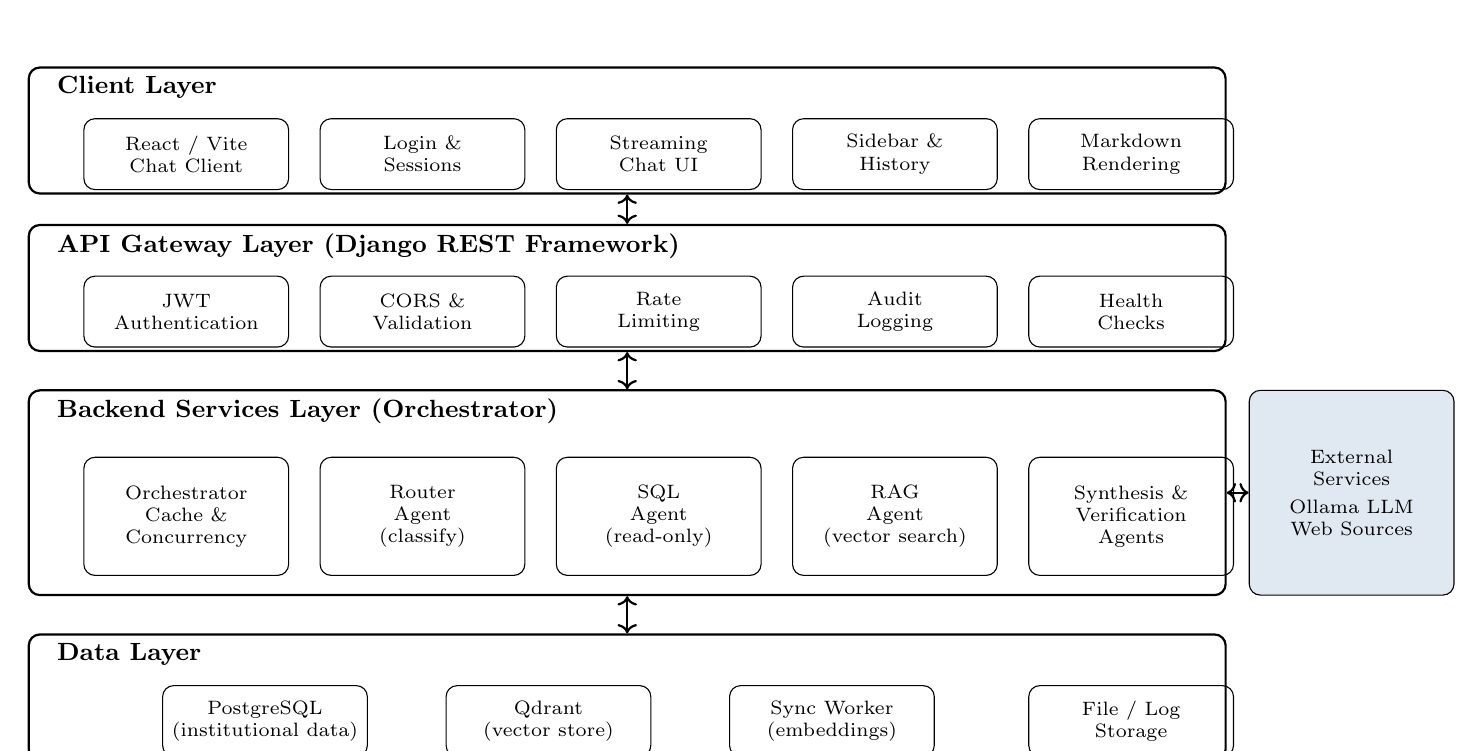
\begin{tikzpicture}[
  layer/.style={draw, rounded corners, thick, minimum width=15.2cm, align=center, font=\bfseries\small},
  box/.style={draw, rounded corners, minimum width=2.6cm, minimum height=0.9cm, align=center, font=\scriptsize},
  extbox/.style={draw, rounded corners, minimum width=2.6cm, minimum height=0.9cm, align=center, font=\scriptsize, fill=hdrblue},
  every node/.style={font=\scriptsize}
]

\node[layer, minimum height=1.6cm] (client) at (0,9.6) {};
\node[anchor=north west, font=\bfseries\small] at (client.north west) {\ \ Client Layer};
\node[box] (webclient) at (-5.6,9.3) {React / Vite\\Chat Client};
\node[box] (login) at (-2.6,9.3) {Login \&\\Sessions};
\node[box] (chatui) at (0.4,9.3) {Streaming\\Chat UI};
\node[box] (sidebar) at (3.4,9.3) {Sidebar \&\\History};
\node[box] (markdown) at (6.4,9.3) {Markdown\\Rendering};

\node[layer, minimum height=1.6cm] (api) at (0,7.6) {};
\node[anchor=north west, font=\bfseries\small] at (api.north west) {\ \ API Gateway Layer (Django REST Framework)};
\node[box] (jwt) at (-5.6,7.3) {JWT\\Authentication};
\node[box] (cors) at (-2.6,7.3) {CORS \&\\Validation};
\node[box] (throttle) at (0.4,7.3) {Rate\\Limiting};
\node[box] (audit) at (3.4,7.3) {Audit\\Logging};
\node[box] (health) at (6.4,7.3) {Health\\Checks};

\node[layer, minimum height=2.6cm] (backend) at (0,5) {};
\node[anchor=north west, font=\bfseries\small] at (backend.north west) {\ \ Backend Services Layer (Orchestrator)};
\node[box, minimum height=1.5cm] (orch) at (-5.6,4.7) {Orchestrator\\Cache \&\\Concurrency};
\node[box, minimum height=1.5cm] (router) at (-2.6,4.7) {Router\\Agent\\(classify)};
\node[box, minimum height=1.5cm] (sql) at (0.4,4.7) {SQL\\Agent\\(read-only)};
\node[box, minimum height=1.5cm] (rag) at (3.4,4.7) {RAG\\Agent\\(vector search)};
\node[box, minimum height=1.5cm] (synth) at (6.4,4.7) {Synthesis \&\\Verification\\Agents};

\node[extbox, minimum height=2.6cm] (ext) at (9.2,5) {External\\Services\\[2pt]Ollama LLM\\Web Sources};

\node[layer, minimum height=1.6cm] (data) at (0,2.4) {};
\node[anchor=north west, font=\bfseries\small] at (data.north west) {\ \ Data Layer};
\node[box] (pg) at (-4.6,2.1) {PostgreSQL\\(institutional data)};
\node[box] (qdrant) at (-1.0,2.1) {Qdrant\\(vector store)};
\node[box] (syncw) at (2.6,2.1) {Sync Worker\\(embeddings)};
\node[box] (files) at (6.4,2.1) {File / Log\\Storage};

\draw[<->, thick] (client.south) -- (api.north);
\draw[<->, thick] (api.south) -- (backend.north);
\draw[<->, thick] (backend.east) -- (ext.west);
\draw[<->, thick] (backend.south) -- (data.north);

\end{tikzpicture}
\caption{Layered system architecture}
\label{fig:arch}
\end{figure}

\section{Agent Pipeline and Request Lifecycle}

Figure~\ref{fig:pipeline} traces a single question through the system.
The router first classifies the question into one of four routes ---
\texttt{SQL}, \texttt{RAG}, \texttt{BOTH}, or \texttt{WEB} --- using a fast,
rule-and-embedding-based classifier (Section~5.3) rather than a full LLM call.
Depending on the route, the SQL agent, the RAG agent, or the web-fetch agent
(or a combination) gathers evidence; the synthesis agent then composes a
natural-language answer from that evidence and streams it to the client
token-by-token; and the verification agent independently checks the streamed
answer against the evidence it was given before the response is marked
complete. If a downstream source is unavailable, the orchestrator degrades
gracefully and annotates the answer rather than failing the request outright
(Section~5.2).

\begin{figure}[h]
\centering
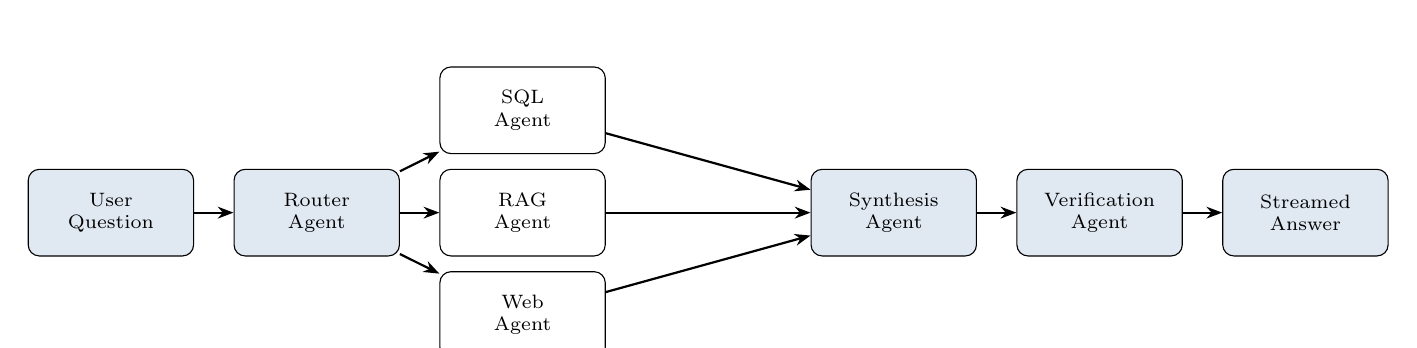
\begin{tikzpicture}[
  node distance=0.5cm and 0.5cm,
  every node/.style={font=\scriptsize},
  stepbox/.style={draw, rounded corners, minimum width=2.1cm, minimum height=1.1cm, align=center, fill=hdrblue},
  decbox/.style={draw, rounded corners, minimum width=2.1cm, minimum height=1.1cm, align=center}
]
\node[stepbox] (user) {User\\Question};
\node[stepbox, right=of user] (router) {Router\\Agent};
\node[decbox, right=of router, yshift=1.3cm] (sqlbox) {SQL\\Agent};
\node[decbox, right=of router] (ragbox) {RAG\\Agent};
\node[decbox, right=of router, yshift=-1.3cm] (webbox) {Web\\Agent};
\node[stepbox, right=2.6cm of ragbox] (synth) {Synthesis\\Agent};
\node[stepbox, right=of synth] (verify) {Verification\\Agent};
\node[stepbox, right=of verify] (out) {Streamed\\Answer};

\draw[-{Stealth[length=2mm]}, thick] (user) -- (router);
\draw[-{Stealth[length=2mm]}, thick] (router) -- (sqlbox);
\draw[-{Stealth[length=2mm]}, thick] (router) -- (ragbox);
\draw[-{Stealth[length=2mm]}, thick] (router) -- (webbox);
\draw[-{Stealth[length=2mm]}, thick] (sqlbox) -- (synth);
\draw[-{Stealth[length=2mm]}, thick] (ragbox) -- (synth);
\draw[-{Stealth[length=2mm]}, thick] (webbox) -- (synth);
\draw[-{Stealth[length=2mm]}, thick] (synth) -- (verify);
\draw[-{Stealth[length=2mm]}, thick] (verify) -- (out);
\end{tikzpicture}
\caption{Agent pipeline for a single request}
\label{fig:pipeline}
\end{figure}

\section{Data Layer}

Structured institutional data lives in PostgreSQL. The language model reaches
it only through a dedicated read-only role, \texttt{rag\_agent\_ro}, granted
\texttt{SELECT} on 12 named tables covering courses, departments, faculty,
fee schedules, and timetables; tables holding per-student records
(\texttt{students}, \texttt{enrollments}, \texttt{exam\_results},
\texttt{fee\_payments}, \texttt{attendance}) and tables holding credentials or
conversation history are not granted to this role at all, so they are
unreachable through the AI pipeline regardless of what SQL the model
generates (Section~5.4 and Section~4.4 detail the enforcement).

Descriptive content --- institutional documents, policies, and other
free-text material --- is embedded with \texttt{nomic-embed-text} and stored
in a Qdrant collection. A background sync worker watches a change queue on
the relational database, converts changed rows to text, generates embeddings,
and upserts them into Qdrant, so the vector index stays consistent with the
system of record without requiring a full reindex on every update.

\section{Security Architecture}

Three controls hold even if the language model itself is fully subverted by a
prompt-injection attack, because they do not depend on the model behaving
correctly:

\begin{enumerate}
\item \textbf{Read-only, schema-restricted database role.} Every SQL
      statement the model causes to run executes under
      \texttt{rag\_agent\_ro}, which has \texttt{default\_transaction\_
      read\_only} set at the role level (so writes are blocked before
      privileges are even checked), is granted \texttt{SELECT} on 12
      non-sensitive tables only, and carries \texttt{NOSUPERUSER
      NOCREATEDB NOCREATEROLE} and a connection limit of 10.
\item \textbf{Independent SQL validation.} Generated SQL is parsed with
      \texttt{sqlglot} and rejected unless it is a single, capped
      \texttt{SELECT} statement referencing only allow-listed tables, with
      results capped at 50 rows. The check is token-level rather than
      regex-based, so a course literally titled ``Update Systems'' is not
      mistaken for an \texttt{UPDATE} statement.
\item \textbf{No model-chosen URLs.} The web-fetch agent selects from a
      fixed \texttt{urls\_allowlist.json} by deterministic keyword matching.
      The model is never asked for, and cannot supply, a URL. Matching is
      exact-string (so a look-alike domain is rejected), redirects are
      followed manually with every hop re-checked, and DNS results are
      checked so an allow-listed hostname resolving to a private or
      link-local address --- including the cloud metadata address
      \texttt{169.254.169.254} --- is refused.
\end{enumerate}

Around these three structural controls sits a conventional application
security layer: PBKDF2-hashed passwords with a 12-character minimum and
common-password rejection, a 30-minute idle session timeout, per-user and
per-IP rate limiting, and account lockout after five failed attempts,
described further in Section~5.9.

\section{Deployment Architecture}

The system is defined as a single Docker Compose stack with the services
listed in Table~\ref{tab:services}. Each service exposes a health-check
endpoint, and the backend will not report healthy until its dependencies
(database, vector store, LLM runtime) are themselves reachable.

\begin{table}[h]
\centering
\caption{Docker Compose services}
\label{tab:services}
\renewcommand{\arraystretch}{1.3}
\begin{tabularx}{\linewidth}{|>{\bfseries}p{2.6cm}|X|}
\hline
\rowcolor{hdrnavy}
\textcolor{white}{Service} & \textcolor{white}{Role} \\
\hline
postgres & Relational database holding institutional data and application
  state. \\
\hline
qdrant & Vector database for descriptive-content retrieval. \\
\hline
ollama / ollama-pull & Local LLM runtime; \texttt{ollama-pull} fetches the
  configured models on first start. \\
\hline
backend & Django REST Framework API, orchestrator, and all five agents. \\
\hline
sync\_worker & Keeps the Qdrant index consistent with PostgreSQL. \\
\hline
caddy & Reverse proxy issuing local (development) or automatic
  (production) TLS certificates. \\
\hline
\end{tabularx}
\end{table}

% =====================================================================
% CHAPTER 5 -- IMPLEMENTATION
% =====================================================================
\chapter{Implementation}

\section{Technology Stack}

\begin{table}[h]
\centering
\caption{Technology stack}
\renewcommand{\arraystretch}{1.3}
\begin{tabularx}{\linewidth}{|>{\bfseries}p{3.2cm}|X|}
\hline
\rowcolor{hdrnavy}
\textcolor{white}{Layer} & \textcolor{white}{Technology} \\
\hline
Backend framework & Python 3.12, Django, Django REST Framework \\
\hline
Frontend & React, Vite, Tailwind CSS \\
\hline
Relational database & PostgreSQL \\
\hline
Vector database & Qdrant \\
\hline
LLM runtime & Ollama, serving \texttt{qwen2.5:7b} (generation) and
  \texttt{nomic-embed-text} (embeddings) \\
\hline
SQL validation & \texttt{sqlglot} \\
\hline
Auth \& sessions & Django's PBKDF2-SHA256 hashing, JWT, DRF throttling \\
\hline
Reverse proxy / TLS & Caddy \\
\hline
Containerisation & Docker, Docker Compose \\
\hline
\end{tabularx}
\end{table}

\section{Orchestrator}

The orchestrator (\texttt{orchestrator/service.py}) is the entry point for
every question. It resolves a route by calling the router agent, dispatches
to the SQL, RAG, and/or web agents concurrently using a thread pool, applies a
concurrency guard (\texttt{llm\_slot}) so the number of simultaneous LLM
calls stays within what the resident models can serve, checks a semantic
cache before generating, and appends a degradation note to the answer --- for
example, \emph{``live records lookup is temporarily unavailable, so this
answer is based on descriptive information only''} --- when one evidence
source is down but the system can still answer from the other rather than
failing the whole request.

\section{Router Agent}

The router agent (\texttt{router\_agent/classifier.py}) decides between the
\texttt{SQL}, \texttt{RAG}, \texttt{BOTH}, and \texttt{WEB} routes. The
original implementation asked a 7-billion-parameter model to classify each
question from a roughly 1,200-token few-shot prompt, which Chapter~7 shows
cost 5.7 seconds per question for a decision worth about twenty tokens of
JSON. It was replaced with a rule-and-embedding based classifier that makes
the same decision in well under a millisecond with no measured change in
routing accuracy on a 29-question labelled evaluation set.

\section{SQL Agent and Guard}

The SQL agent (\texttt{sql\_agent/service.py}) prompts the LLM with the
allow-listed schema and the user's question, and receives a candidate SQL
statement back. That statement is never executed directly. It first passes
through \texttt{sql\_agent/guard.py}, which:

\begin{itemize}[leftmargin=1.5em]
\item parses the statement with \texttt{sqlglot} rather than matching it
      against a regular expression, so that a string literal containing a
      keyword like \texttt{UPDATE} is not mistaken for the keyword itself;
\item rejects anything that is not a single \texttt{SELECT} statement, any
      table outside the allow-list, and any of the forbidden keyword tokens
      \texttt{INSERT}, \texttt{UPDATE}, \texttt{DELETE}, \texttt{DROP}, and
      \texttt{ALTER};
\item caps the result set at 50 rows.
\end{itemize}

Only a statement that survives the guard is executed, and it is executed
under the read-only \texttt{rag\_agent\_ro} role described in Section~4.4, so
even a guard bypass would still be bounded by what that role can read.

\section{RAG Agent}

The RAG agent (\texttt{rag\_agent/service.py},
\texttt{rag\_agent/vector\_store.py}) embeds the incoming question with
\texttt{nomic-embed-text} and retrieves the top-$k$ ($k=5$) nearest passages
from the Qdrant collection populated by the sync worker. Retrieved passages
are passed to the synthesis agent as evidence rather than being shown to the
user directly.

\section{Synthesis and Verification Agents}

The synthesis agent (\texttt{synthesis\_agent/service.py}) composes the final
answer from whatever evidence the SQL, RAG, and/or web agents produced,
streaming tokens to the client as they are generated
(\texttt{synthesize\_answer\_stream}). The verification agent then checks the
completed answer against the same evidence before the response is marked
final. For short, low-claim-count answers (typically SQL-sourced), a
no-LLM fast path performs this check directly, which Chapter~7 shows cut
verification latency for that case from 11.3 seconds to 50 milliseconds; for
longer, evidence-dense answers a terse-verdict LLM call is still used, but a
more compact verdict format alone brought RAG-answer verification down from
168.5 seconds to 62.3 seconds.

\section{Web Agent}

The web agent (\texttt{web\_agent/service.py}) is consulted only for
questions matched by keyword to a fixed \texttt{urls\_allowlist.json} of
official institutional pages. As noted in Section~4.4, the model never
supplies a URL; the agent selects one deterministically. Fourteen tests in
\texttt{web\_agent/tests.py} cover this path, including live refusal of
internal service addresses (\texttt{ollama:11434}, \texttt{postgres:5432},
\texttt{qdrant:6333}), the cloud metadata address, and \texttt{file://} URIs.

\section{Frontend}

The client is a React application built with Vite, using Tailwind CSS for
styling and \texttt{react-markdown} with \texttt{rehype-highlight} to render
streamed answers, including code blocks, as they arrive. It authenticates
against the Django backend, maintains conversation history per user, and
renders the same degradation notes the orchestrator attaches when an
evidence source was unavailable, so the limitation is visible to the user
rather than silently hidden.

\section{Authentication and Session Management}

Authentication combines an institutional email/password login with
JWT-based API sessions. Passwords are hashed with Django's default PBKDF2-
SHA256, must be at least 12 characters, and are checked against a list of
roughly 20,000 common passwords and against similarity to the user's own
name, username, and email. Sessions expire after 30 minutes of inactivity and
on browser close; session cookies are \texttt{HttpOnly}, \texttt{Secure}, and
\texttt{SameSite=Lax}. Login is rate-limited to 10 attempts per minute per
IP address, and, independently, an account is locked for 15 minutes after
five consecutive failed attempts against it --- a control that matters
because it bounds guesses against one account regardless of how many source
IP addresses an attacker distributes the attempt across, which a purely
per-IP limit cannot do. During the security review documented in
Chapter~6, the login endpoint was found to be exempt from CSRF protection
(a consequence of Django REST Framework marking \texttt{@api\_view} views
\texttt{csrf\_exempt} by default) and was fixed before deployment.

\section{Representative Code Excerpt}

Listing~\ref{lst:routecode} shows the route-resolution function from the
orchestrator: it calls the router agent, falls back to answering from both
sources if routing itself fails, and returns both the chosen route and a
human-readable reason that is logged for later audit.

\begin{lstlisting}[caption={Route resolution in the orchestrator (\texttt{orchestrator/service.py})}, label={lst:routecode}]
def _resolve_route(question):
    # classify() can raise LLMUnavailable (Ollama down) -- we let that
    # propagate, since if the LLM is down synthesis can't run either. A
    # *parse* failure (route_result.error) is different: fall back to
    # BOTH and carry on.
    route_result = classify(question)
    if route_result.error:
        logger.warning(
            "router failed question=%r error=%s -- falling back to %s",
            question, route_result.error, DEFAULT_ROUTE_ON_ERROR,
        )
        return DEFAULT_ROUTE_ON_ERROR, (
            f"router error, defaulted to {DEFAULT_ROUTE_ON_ERROR}"
        )
    return route_result.route, route_result.reason
\end{lstlisting}

% =====================================================================
% CHAPTER 6 -- TESTING
% =====================================================================
\chapter{Testing}

\section{Testing Strategy}

Testing was carried out at two levels. Unit and integration tests, run with
Django's test runner, cover each agent's decision logic in isolation
(classification, SQL guard rejections, verification verdicts) and the
authentication flow. Security testing was carried out against the running
system rather than only at the unit level, because the properties that
matter most --- can a write actually reach the database, can the web agent
actually be redirected to an internal address --- are only meaningfully true
if demonstrated against the live stack, not merely asserted in a mock.

\section{Unit Test Coverage}

\begin{table}[h]
\centering
\caption{Unit tests by module}
\renewcommand{\arraystretch}{1.3}
\begin{tabularx}{\linewidth}{|X|r|}
\hline
\rowcolor{hdrnavy}
\textcolor{white}{Module} & \textcolor{white}{Test count} \\
\hline
\texttt{accounts} (authentication, lockout, sessions) & 24 \\
\hline
\texttt{web\_agent} (allowlist, SSRF refusal) & 24 \\
\hline
\texttt{verification\_agent} & 17 \\
\hline
\texttt{synthesis\_agent} & 14 \\
\hline
\texttt{orchestrator} & 13 \\
\hline
\texttt{router\_agent} & 8 \\
\hline
\texttt{sql\_agent} (guard rejections) & 5 \\
\hline
\rowcolor{hdrblue}
\textbf{Total} & \textbf{105} \\
\hline
\end{tabularx}
\end{table}

\section{Security Testing}

Several controls were verified directly against the running system rather
than only through unit tests:

\begin{itemize}[leftmargin=1.5em]
\item \textbf{Read-only role enforcement.} \texttt{manage.py
      check\_rag\_agent\_ro --check-write} attempted a real \texttt{INSERT}
      under the \texttt{rag\_agent\_ro} role; it was rejected with
      \emph{``session is read-only''}. This was re-verified after the
      web-fetch agent and multi-user authentication were added, to confirm
      neither change widened the role's privileges.
\item \textbf{SSRF / URL restriction.} Live requests to
      \texttt{ollama:11434}, \texttt{postgres:5432}, \texttt{qdrant:6333},
      the cloud metadata address \texttt{169.254.169.254}, and a
      \texttt{file:///etc/passwd} URI were all refused by the web agent.
\item \textbf{Brute-force lockout.} Five consecutive failed logins against
      one account triggered a 15-minute lockout, confirmed to persist
      across a backend restart because lockout state is stored on the
      database row rather than in an in-memory cache.
\item \textbf{Login CSRF.} Prior to the fix described in Section~5.9, a
      forged cross-site POST to the login endpoint returned a valid session
      cookie for the attacker's account without a CSRF token; after the
      fix, the same request is rejected.
\end{itemize}

\section{Representative Test Cases}

\begin{table}[h]
\centering
\caption{Representative test cases}
\renewcommand{\arraystretch}{1.4}
\begin{tabularx}{\linewidth}{|>{\raggedright\arraybackslash}p{3.4cm}|X|X|}
\hline
\rowcolor{hdrnavy}
\textcolor{white}{Test} & \textcolor{white}{Input / Action} &
\textcolor{white}{Expected result} \\
\hline
SQL guard, forbidden keyword & Model generates a statement containing
  \texttt{DROP TABLE} & Statement rejected before execution \\
\hline
SQL guard, false-positive keyword & Question about a course titled
  ``Update Systems'' & Statement accepted; \texttt{UPDATE} recognised as a
  string literal, not a keyword \\
\hline
Read-only role & Direct \texttt{INSERT} attempted as
  \texttt{rag\_agent\_ro} & Rejected: session is read-only \\
\hline
Web agent, look-alike domain & Allow-listed \texttt{example.com}
  vs.\ \texttt{example.com.attacker.test} & Look-alike domain rejected \\
\hline
Account lockout & 5 failed logins against one account & 6th attempt
  rejected regardless of source IP; lock persists across restart \\
\hline
Login CSRF (pre-fix) & Forged cross-site POST to \texttt{/api/auth/login/} &
  Valid session issued (vulnerability, since remediated) \\
\hline
Degraded mode & Database made unreachable mid-session & RAG-only answer
  returned with a note that live records were unavailable \\
\hline
\end{tabularx}
\end{table}

% =====================================================================
% CHAPTER 7 -- RESULTS AND PERFORMANCE EVALUATION
% =====================================================================
\chapter{Results and Performance Evaluation}

\section{Experimental Setup}

All measurements in this chapter were taken on an Intel Core Ultra 9 185H
(16 cores / 22 threads), 31.4\,GB RAM, with \textbf{no CUDA GPU} --- a
deliberately conservative choice of hardware, since it represents the lower
bound an institution might actually deploy on rather than a
best-case research machine. On this hardware, Ollama generated at 9.0
tokens/second and read prompts at 44 tokens/second. Per-stage timings were
captured for every request by an always-on profiler
(\texttt{orchestrator/profiling.py}) riding along on the response's
completion event, so the figures below come from the real API rather than a
synthetic benchmark harness.

\section{Latency Optimisation}

Table~\ref{tab:latency} summarises the effect of two targeted changes: replacing
the LLM-based router with the rule-and-embedding classifier of
Section~5.3, and introducing a no-LLM fast path plus a terser verdict format
for verification (Section~5.6). The same seven questions, in the same order,
were run against the backend before and after the change, with the backend
restarted between runs.

\begin{table}[h]
\centering
\caption{Latency before and after optimisation}
\label{tab:latency}
\renewcommand{\arraystretch}{1.3}
\begin{tabular}{|l|r|r|r|}
\hline
\rowcolor{hdrnavy}
\textcolor{white}{Stage} & \textcolor{white}{Before} &
\textcolor{white}{After} & \textcolor{white}{Improvement} \\
\hline
Router & 5{,}742\,ms & 0.4\,ms & $\sim$14{,}000$\times$ \\
\hline
Verification (SQL answers) & 11{,}270\,ms & 50\,ms & 225$\times$ \\
\hline
Verification (RAG answers) & 168{,}485\,ms & 62{,}314\,ms & 2.7$\times$ \\
\hline
Time to first token & 79.8\,s & 46.8\,s & 1.7$\times$ \\
\hline
\rowcolor{hdrblue}
End-to-end, 7 questions & 1{,}455.8\,s & 876.7\,s & 1.66$\times$ \\
\hline
\end{tabular}
\end{table}

Routing accuracy did not move: both runs produced identical routes on all
seven questions, and a separate 29-question labelled evaluation set measured
100\% precision at 97\% coverage for the new classifier. No answer was
truncated by the change; the longest answer observed was 1,252 characters
against a roughly 3,500-character cap. Synthesis time itself was essentially
unchanged (76.1\,s to 78.5\,s median) and two of the seven questions were
individually slower after the change, entirely from run-to-run synthesis
variance --- CPU-bound generation time was observed to vary by up to $\pm$30\%
between otherwise identical runs, so single-run synthesis figures should be
read with that caveat; the router and verification improvements, changing by
two to four orders of magnitude, are not subject to the same noise.

\section{Where the Latency Actually Goes}

A separate single-question profile (Table~\ref{tab:profile}), taken with all
models already resident in memory, shows that LLM inference dominates the
pipeline and the database does not.

\begin{table}[h]
\centering
\caption{Per-stage share of latency, warm models, single SQL question}
\label{tab:profile}
\renewcommand{\arraystretch}{1.3}
\begin{tabular}{|l|r|r|}
\hline
\rowcolor{hdrnavy}
\textcolor{white}{Stage} & \textcolor{white}{Time} & \textcolor{white}{Share} \\
\hline
Verification (LLM) & 5.17\,s & 27\% \\
\hline
Router classify (LLM, pre-optimisation) & 3.29\,s & 17\% \\
\hline
SQL generate + execute (LLM) & 2.72\,s & 14\% \\
\hline
Synthesis stream (LLM) & 2.61\,s & 14\% \\
\hline
Qdrant vector search & 0.18\,s & 1\% \\
\hline
Database: schema introspection & 0.02\,s & 0.1\% \\
\hline
Database: connect & 0.01\,s & 0.0\% \\
\hline
Database: execute agent query & 0.00\,s & 0.0\% \\
\hline
\rowcolor{hdrblue}
\textbf{Total LLM share} & & \textbf{72.5\%} \\
\hline
\end{tabular}
\end{table}

The conclusion drawn from this profile is that further database tuning has
essentially nothing left to win --- the database accounts for roughly 0.1\%
of pipeline time --- and that any further latency work should target LLM
inference itself, which the two findings below address.

\section{Model Eviction and Concurrency Findings}

\subsection{Model residency dominates single-request latency}
Ollama's default \texttt{keep\_alive} unloads an idle model after five
minutes; the next question then pays a full reload from disk. On identical
hardware and an identical question, a warm (resident) model answered in
13.46\,s (6.96\,s to first token); a cold (evicted) model took 263.44\,s
(225.69\,s to first token) --- a 19.6$\times$ slowdown. Because the reference
deployment is lightly used outside peak hours, five minutes of quiet between
questions is common, meaning most questions in an unoptimised deployment
would pay this cost. Setting \texttt{OLLAMA\_KEEP\_ALIVE=-1} to keep all
three models resident (at a cost of roughly 7.7\,GB RAM) was, on its own, the
single largest latency improvement made in this project --- larger than the
router and verification optimisations combined.

\subsection{A cache alone does not survive simultaneous identical questions}
Table~\ref{tab:coalescing} shows a 50-simulated-user load test drawing from 5
common questions. A semantic answer cache alone served only 2 of 50 requests,
because every user's request reached the cache lookup before the first
answer had finished generating --- a cache stampede that no similarity
threshold can fix. Adding request coalescing, so that only the first caller
of a given question generates an answer and every later identical request
waits on that in-flight result, raised throughput roughly 7.7$\times$; tuning
the queue timeout on top of that let all 50 requests succeed.

\begin{table}[h]
\centering
\caption{Effect of request coalescing under concurrent load (50 users, 5 questions)}
\label{tab:coalescing}
\renewcommand{\arraystretch}{1.3}
\begin{tabular}{|l|r|r|r|}
\hline
\rowcolor{hdrnavy}
\textcolor{white}{Configuration} & \textcolor{white}{Served} &
\textcolor{white}{Busy / failed} & \textcolor{white}{Throughput} \\
\hline
Cache only & 2 & 48 & 2.4/min \\
\hline
+ Request coalescing & 21 & 29 & 18.4/min \\
\hline
\rowcolor{hdrblue}
+ Tuned queue timeout & \textbf{50} & \textbf{0} & \textbf{28.1/min} \\
\hline
\end{tabular}
\end{table}

\section{Discussion}

Two findings generalise beyond this specific deployment. First, in a
multi-agent pipeline built around a single shared LLM runtime, the agent that
looks cheapest to build --- a router doing a simple four-way classification
--- can dominate cost if implemented as a full LLM call, and is often the
easiest agent to replace with a much cheaper method without a measurable
accuracy loss, as Section~5.3 showed. Second, caching alone is not a
sufficient concurrency strategy for an LLM-backed service; without request
coalescing, a cache only helps requests that arrive strictly after the
answer they want already exists, which is close to never true under
simultaneous load.

\section{Limitations}

RAG-answer verification, at 62.3 seconds median after optimisation, remains
the largest single remaining stage and the main target for further work.
Synthesis time on CPU-only hardware is noisy enough ($\pm$30\% run-to-run)
that single-run comparisons of synthesis latency specifically should not be
over-interpreted; the router and verification results in this chapter are
trusted because they moved by two to four orders of magnitude, well outside
that noise band. All performance figures in this chapter are from one
representative hardware configuration; behaviour on GPU-accelerated hardware
was not measured and is identified as future work in Chapter~8.

% =====================================================================
% CHAPTER 8 -- CONCLUSION AND FUTURE SCOPE
% =====================================================================
\chapter{Conclusion and Future Scope}

\section{Conclusion}

This project set out to answer whether a university could offer a
conversational, natural-language interface to its live institutional data
without sending that data to a cloud service and without granting a language
model unsupervised write or broad read access to its database. The system
built and evaluated in this report answers both questions affirmatively. All
inference --- routing, SQL generation, retrieval, synthesis, and
verification --- runs locally through Ollama; the database role available to
the model is read-only and limited to 12 non-sensitive tables, independently
enforced both by SQL parsing and by database role privileges; and the
web-fetch path can never be pointed at an attacker-chosen or internal
address. Measured on CPU-only commodity hardware, targeted optimisation of
the router and verification stages cut end-to-end median latency for a
seven-question benchmark by 40\%, and a separate scaling study showed the
system, once model residency and request coalescing were addressed, serving
all 50 simulated concurrent users of a shared-question workload rather than
the 2 it served initially. Taken together, the results support the
project's central claim: a defence-in-depth, multi-agent architecture is a
practical way to give an institution conversational access to its own data
without a cloud dependency and without trusting the language model itself
with anything it should not have.

\section{Future Scope}

\begin{itemize}[leftmargin=1.5em]
\item \textbf{GPU-accelerated serving.} Since LLM inference accounts for
      72.5\% of pipeline time on CPU-only hardware, a GPU serving layer is
      the most direct remaining path to lower latency, and is a natural next
      deployment tier above the CPU baseline documented in this report.
\item \textbf{Broader, still-guarded data access.} Additional read-only
      roles, scoped to specific staff or departmental needs, could extend
      coverage beyond the current 12-table allowlist without weakening the
      least-privilege guarantee.
\item \textbf{Adaptive request coalescing.} The queue-timeout tuning in
      Section~7.4 was found empirically; an adaptive scheme that adjusts to
      observed load could remove the need for manual tuning.
\item \textbf{Native mobile client.} The current interface is a responsive
      web client; a native mobile application would extend reach without
      changing the backend architecture.
\item \textbf{Multi-institution deployment templates.} Packaging the
      allow-list, schema mapping, and Compose configuration as a
      per-institution template would reduce the effort required to deploy
      the system at a second institution.
\item \textbf{Formal red-teaming of the verification agent.} The
      verification stage is currently evaluated on correctness and latency;
      a structured adversarial evaluation of how reliably it catches an
      incorrect or fabricated answer would strengthen the safety case made
      in Chapter~4.
\end{itemize}

% =====================================================================
% REFERENCES
% =====================================================================
\begin{thebibliography}{99}

\bibitem{lewis2020rag}
P.~Lewis, E.~Perez, A.~Piktus, F.~Petroni, V.~Karpukhin, N.~Goyal,
H.~K\"uttler, M.~Lewis, W.~Yih, T.~Rockt\"aschel, S.~Riedel, and D.~Kiela,
``Retrieval-Augmented Generation for Knowledge-Intensive NLP Tasks,''
\emph{Advances in Neural Information Processing Systems (NeurIPS)}, 2020.

\bibitem{yu2018spider}
T.~Yu, R.~Zhang, K.~Yang, M.~Yasunaga, D.~Wang, Z.~Li, J.~Ma, I.~Li,
Q.~Yao, S.~Roman, Z.~Zhang, and D.~Radev,
``Spider: A Large-Scale Human-Labeled Dataset for Complex and Cross-Domain
Semantic Parsing and Text-to-SQL Task,'' \emph{Proceedings of EMNLP}, 2018.

\bibitem{yao2023react}
S.~Yao, J.~Zhao, D.~Yu, N.~Du, I.~Shafran, K.~Narasimhan, and Y.~Cao,
``ReAct: Synergizing Reasoning and Acting in Language Models,''
\emph{International Conference on Learning Representations (ICLR)}, 2023.

\bibitem{touvron2023llama}
H.~Touvron, T.~Lavril, G.~Izacard, X.~Martinet, M.-A.~Lachaux, T.~Lacroix,
B.~Rozi\`ere, N.~Goyal, E.~Hambro, F.~Azhar, A.~Rodriguez, A.~Joulin,
E.~Grave, and G.~Lample, ``LLaMA: Open and Efficient Foundation Language
Models,'' \emph{arXiv preprint}, 2023.

\bibitem{qwen2024}
Qwen Team, Alibaba Group, ``Qwen2.5 Technical Report,'' \emph{arXiv
preprint}, 2024.

\bibitem{django}
Django Software Foundation, \emph{Django Documentation}.
\url{https://docs.djangoproject.com}.

\bibitem{postgres}
PostgreSQL Global Development Group, \emph{PostgreSQL Documentation}.
\url{https://www.postgresql.org/docs/}.

\bibitem{qdrant}
Qdrant, \emph{Qdrant Vector Database Documentation}.
\url{https://qdrant.tech/documentation/}.

\bibitem{ollama}
Ollama, \emph{Ollama Documentation}. \url{https://ollama.com}.

\bibitem{dpdpa}
Ministry of Electronics and Information Technology, Government of India,
\emph{Digital Personal Data Protection Act, 2023}.

\bibitem{owasp}
OWASP Foundation, \emph{OWASP Top 10:2021}.
\url{https://owasp.org/Top10/}.

\end{thebibliography}

\end{document}
